%%%%%%%%%%%%%%%%%%%%%%%%%%%%%%%%%%%%%%%%%
% University/School Laboratory Report
% LaTeX Template
% Version 3.1 (25/3/14)
%
% This template has been downloaded from:
% http://www.LaTeXTemplates.com
%
% Original author:
% Linux and Unix Users Group at Virginia Tech Wiki 
% (https://vtluug.org/wiki/Example_LaTeX_chem_lab_report)
%
% License:
% CC BY-NC-SA 3.0 (http://creativecommons.org/licenses/by-nc-sa/3.0/)
%
%%%%%%%%%%%%%%%%%%%%%%%%%%%%%%%%%%%%%%%%%

%----------------------------------------------------------------------------------------
%	PACKAGES AND DOCUMENT CONFIGURATIONS
%----------------------------------------------------------------------------------------

\documentclass{article}

\usepackage{graphicx} % Required for the inclusion of images
\usepackage{amsmath} % Required for some math elements 
\usepackage{cite}
\usepackage{subcaption} %Required to group figures
\usepackage{float}

\setlength\parindent{0pt} % Removes all indentation from paragraphs

%\usepackage{times} % Uncomment to use the Times New Roman font

%----------------------------------------------------------------------------------------
%	DOCUMENT INFORMATION
%----------------------------------------------------------------------------------------

\title{Lab 5\\ Baseband PAM\\ EE 445S} % Title

\author{Enoc Balderas\\
        \and
        Daniel Diamont\\} % Author name

\date{\today} % Date for the report

\begin{document}

\maketitle % Insert the title, author and date

\begin{center}
\begin{tabular}{l r}
Date Performed: & March 1, 2019 \\ % Date the experiment was performed
Instructor: & Professor Evans % Instructor/supervisor
\end{tabular}
\end{center}

% If you wish to include an abstract, uncomment the lines below
% \begin{abstract}
% Abstract text
% \end{abstract}

%----------------------------------------------------------------------------------------
%	SECTION 1
%----------------------------------------------------------------------------------------

\section{Introduction}

In this lab, we investigated aspects of pulse amplitude modulation (PAM) for baseband transmission and reception. The lab was split up into the following three parts: pulse shaping, symbol clock recovery, and demodulation.

\subsection{Pulse Shaping}
Pulse shaping refers in this case to applying a band-limited pulse to an impulse train of symbol amplitudes before sending the signal to the DAC. In this lab, we explored the effects of using differently parametrized raised cosine pulses on the time domain representation of the signal, as well as the effects on quantization.

Specifically, since the raised cosine pulse shape with $ \beta = 1 $ has most of its power in the time domain inside of of the symbol period, then it follows that using the raised cosine to shape successive symbol amplitudes causes less inter symbol interference (ISI). In contrast, using a raised cosine with $ \beta = 0.125, $ which has more power leakage across time with respect to the previous example, then it follows that there will be more inter symbol interference. We can see the difference in ISI by comparing the eye diagrams in Figure 3 and Figure 4. It is clear that we would be able correctly quantize with a higher probability data using a raised cosine with $ \beta = 1 $ as opposed to data using raised cosine with $ \beta = 0.125. $

\subsection{SCR}


\subsection{Demodulation}


%----------------------------------------------------------------------------------------
%	SECTION 2
%----------------------------------------------------------------------------------------

\section{Methods}

%----------------------------------------------------------------------------------------
%	SECTION 3
%----------------------------------------------------------------------------------------

\section{Results}

\subsection{Pulse Shaping}

\begin{figure}[h]
  \begin{center}
    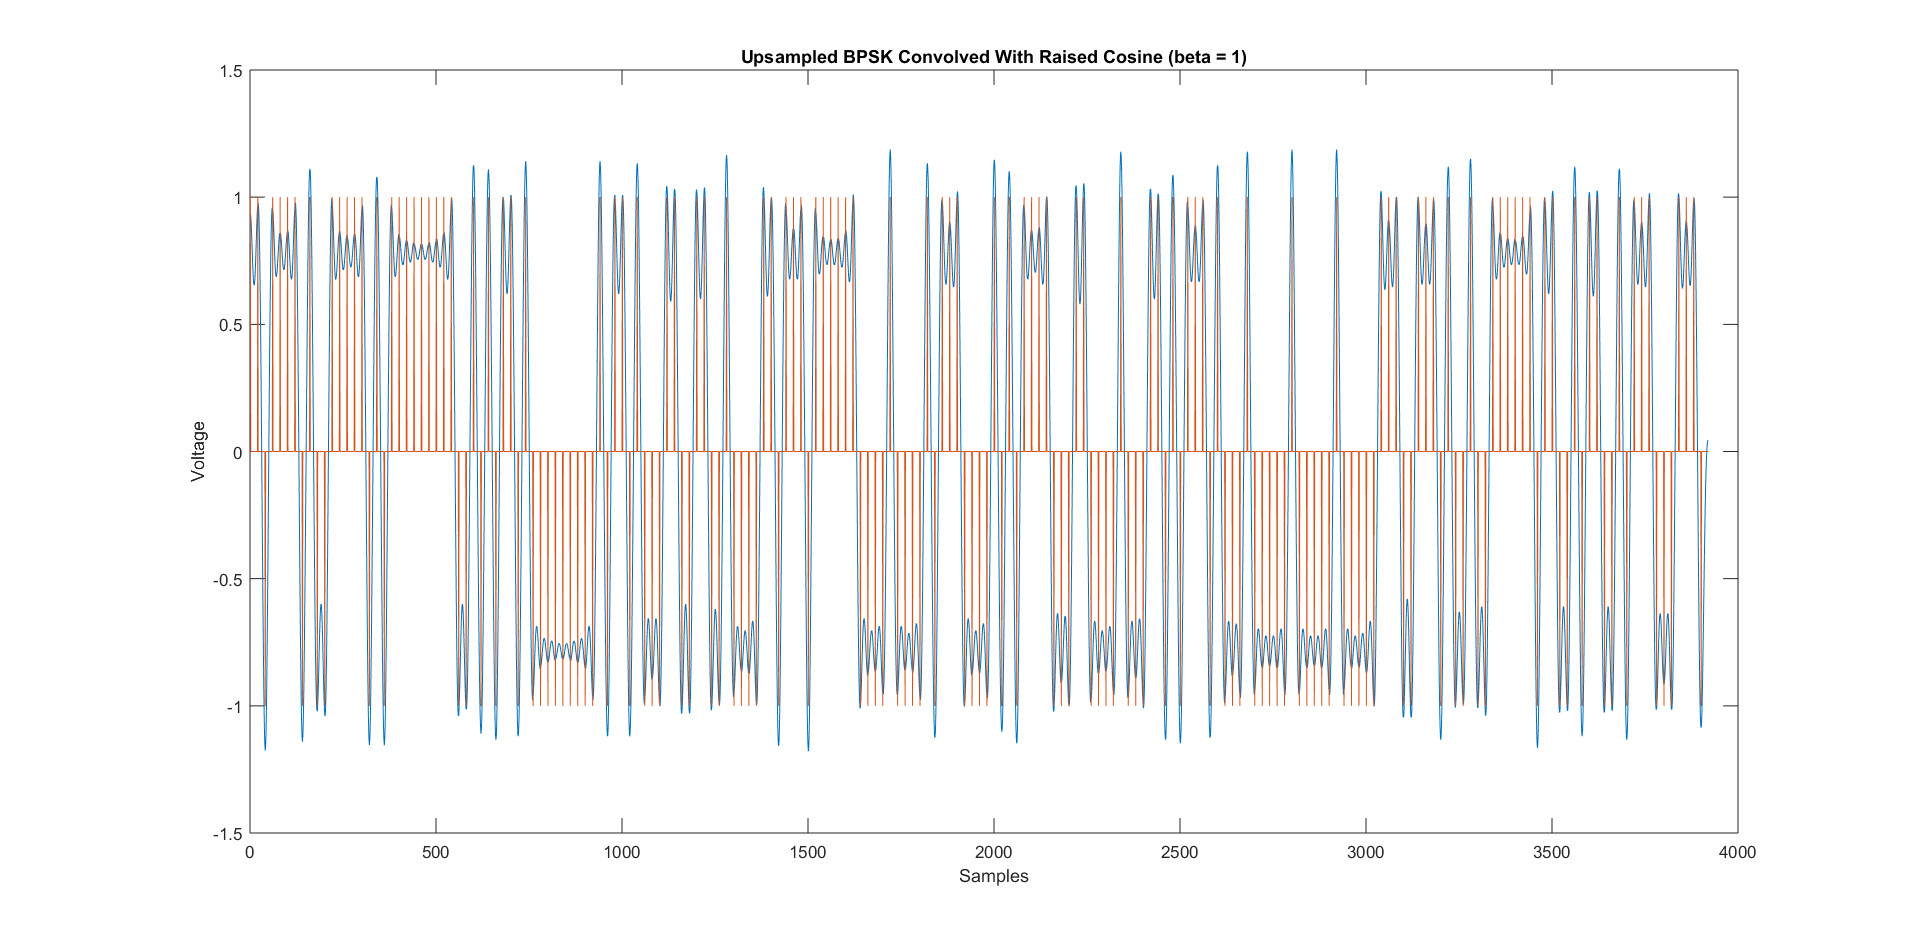
\includegraphics[width=0.65\textwidth]{img/upsampled_bpsk_raised_cosine_beta_1.png}
    \caption{Pulse shape BPSK $\beta = 1$.}
  \end{center}
\end{figure}

\begin{figure}[h]
  \begin{center}
    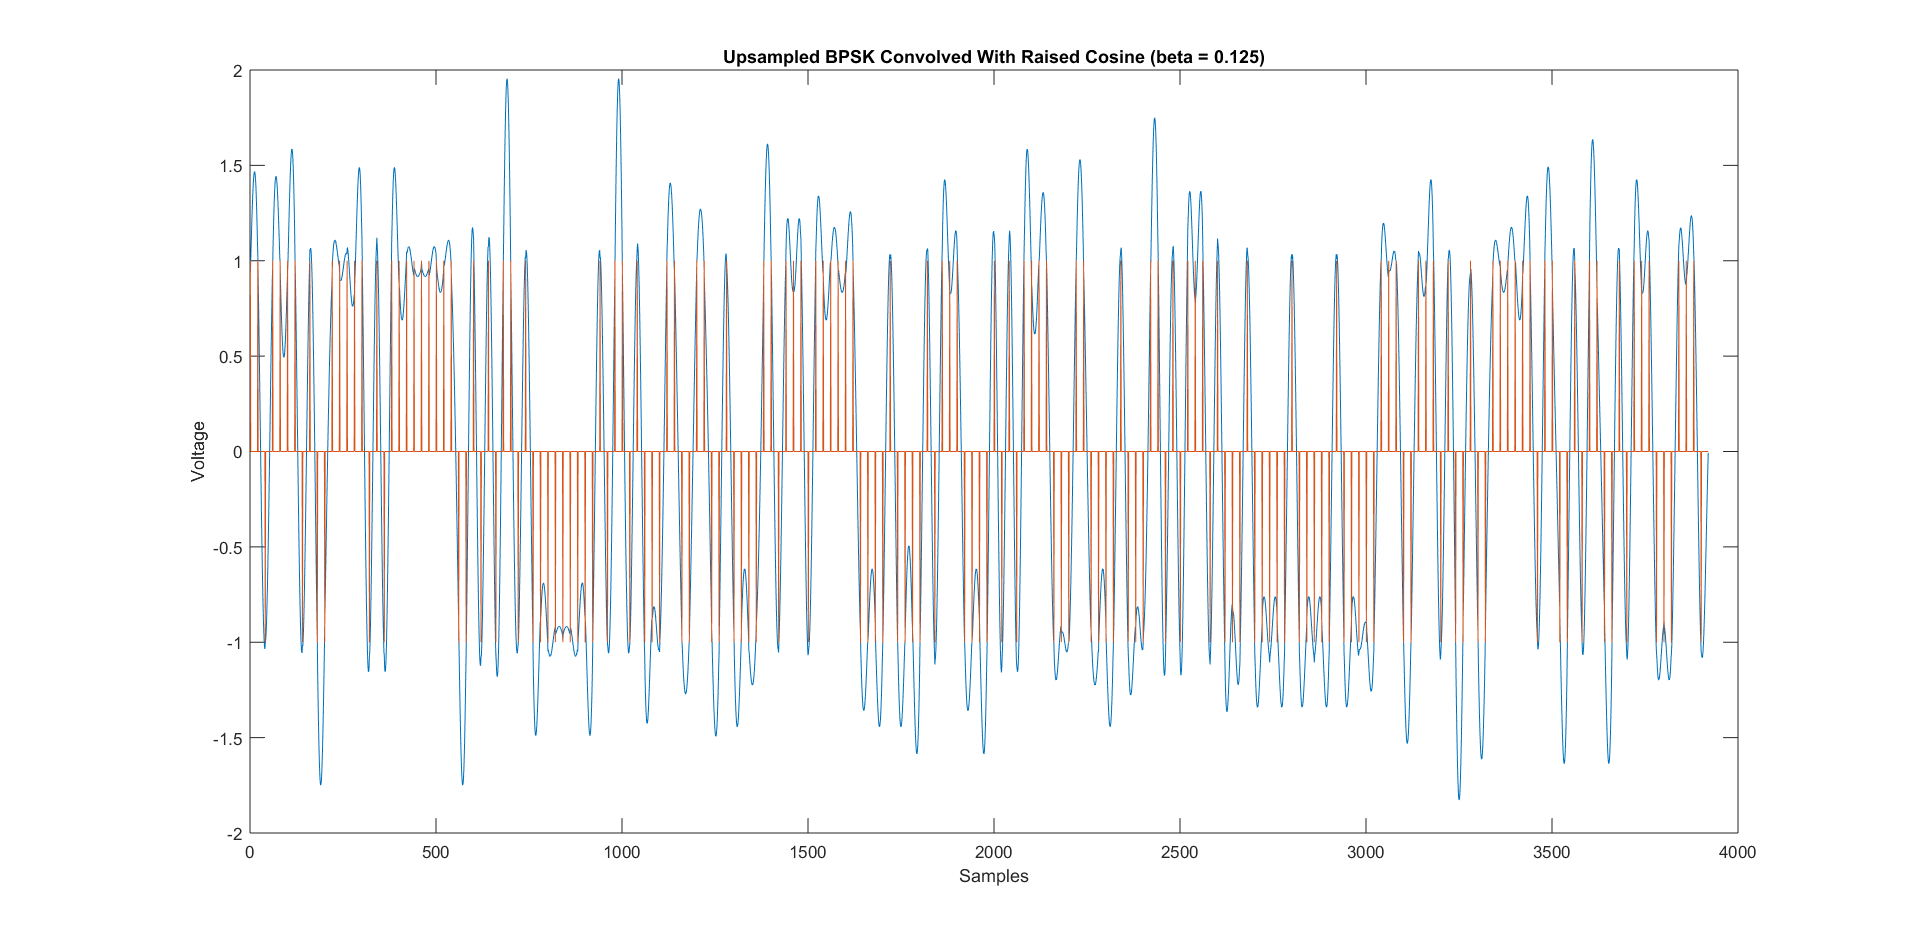
\includegraphics[width=0.65\textwidth]{img/upsampled_bpsk_raised_cosine_beta_125.png}
    \caption{Pulse shape BPSK $\beta = 0.125$.}
  \end{center}
\end{figure}

\begin{figure}[h]
  \begin{center}
    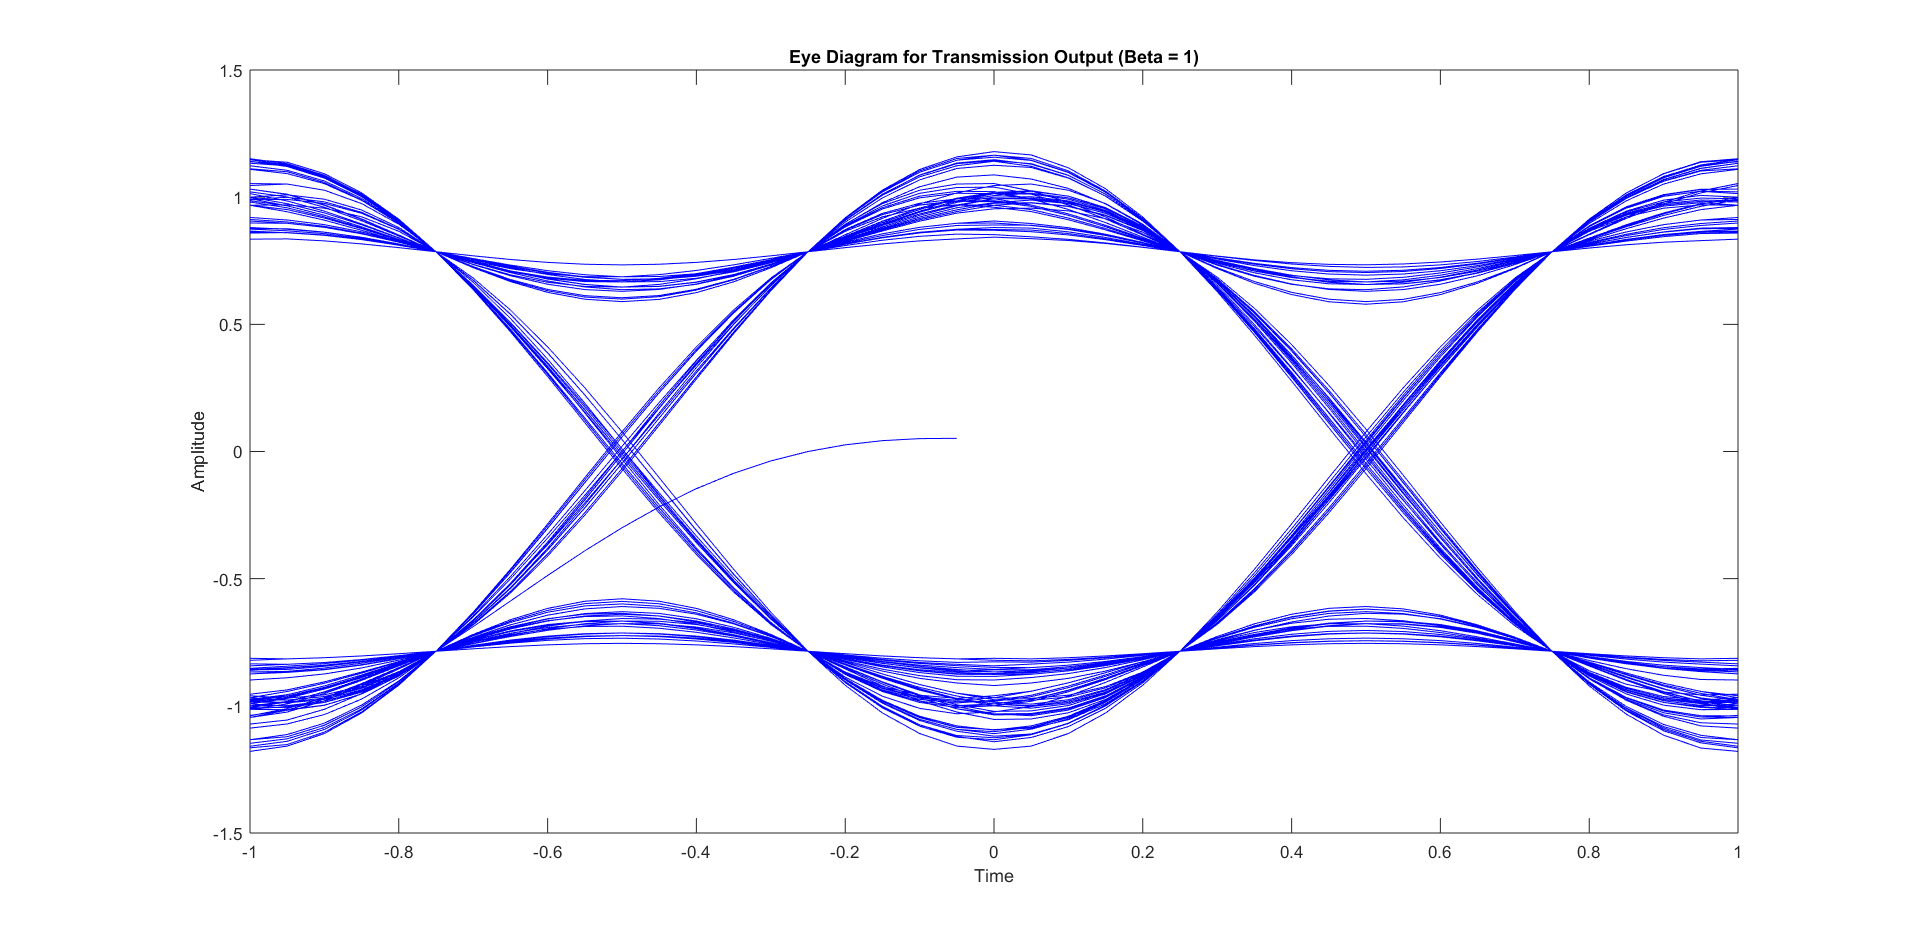
\includegraphics[width=0.65\textwidth]{img/eye_diagram_beta_1.png}
    \caption{Eye diagram $\beta = 1$}
  \end{center}
\end{figure}

\begin{figure}[h]
  \begin{center}
    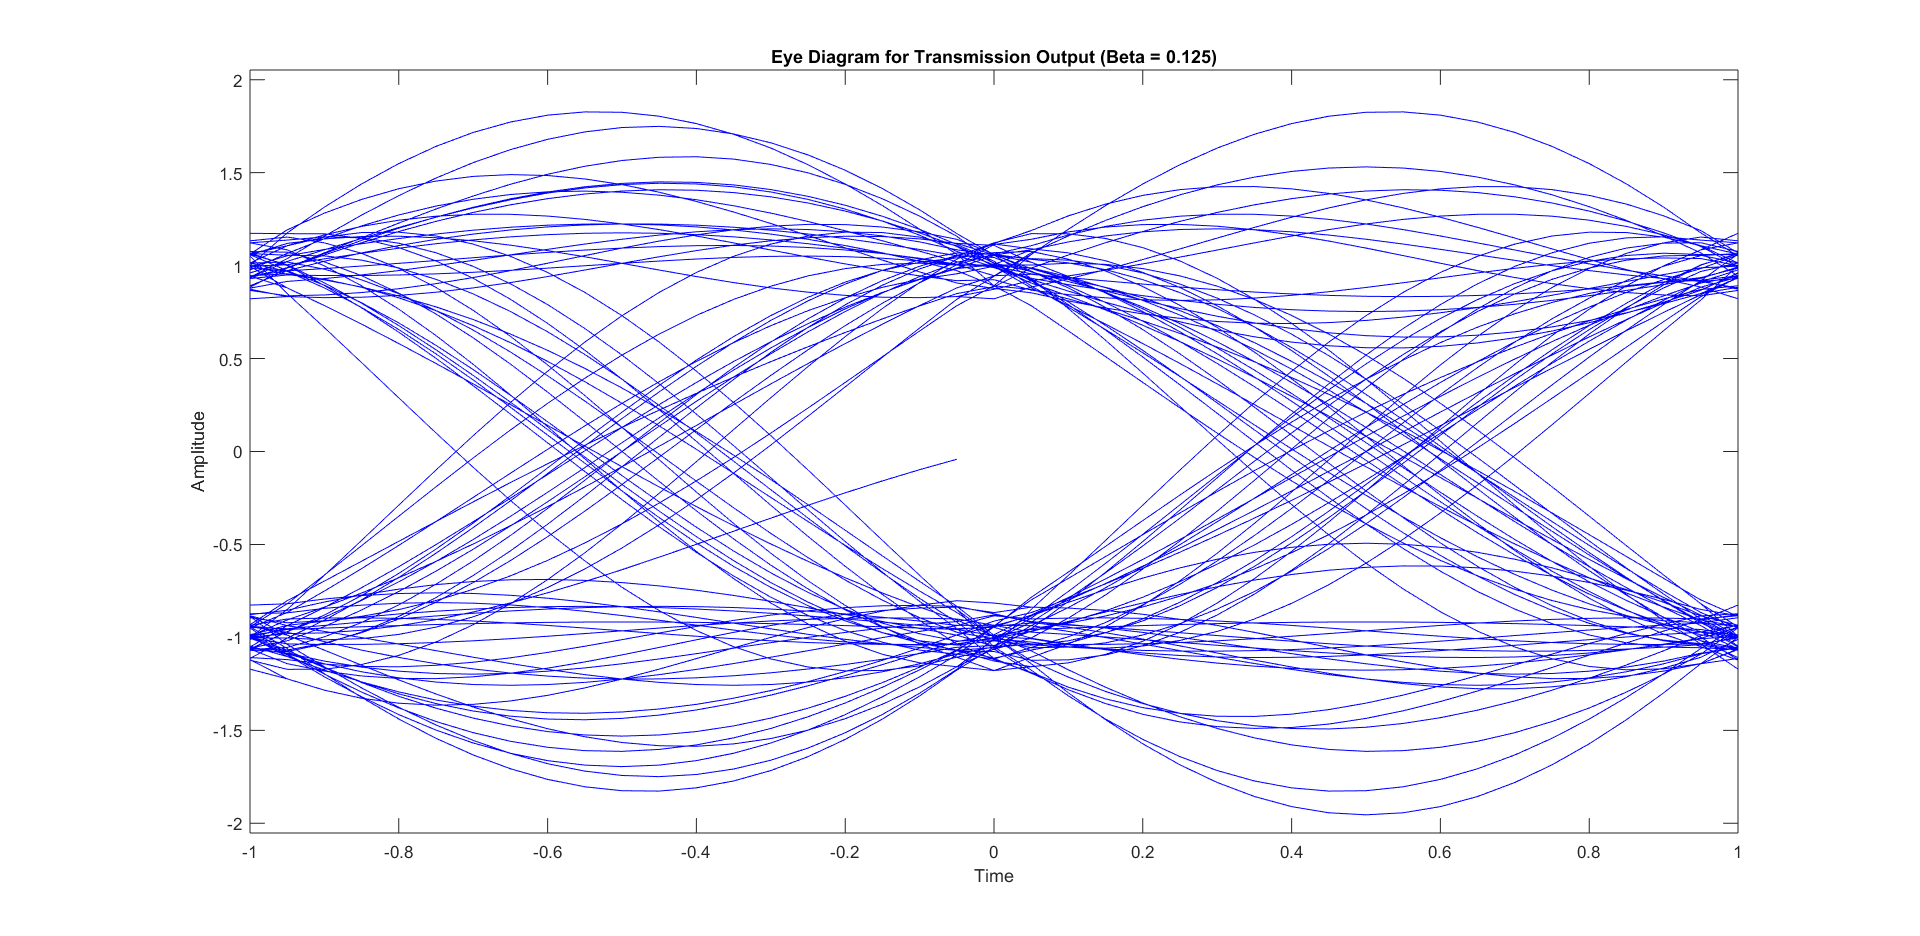
\includegraphics[width=0.65\textwidth]{img/eye_diagram_beta_125.png}
    \caption{Eye diagram $\beta = 0.125$}
  \end{center}
\end{figure}

\begin{figure}[h]
  \begin{center}

    \begin{subfigure}[b]{0.5\linewidth}
      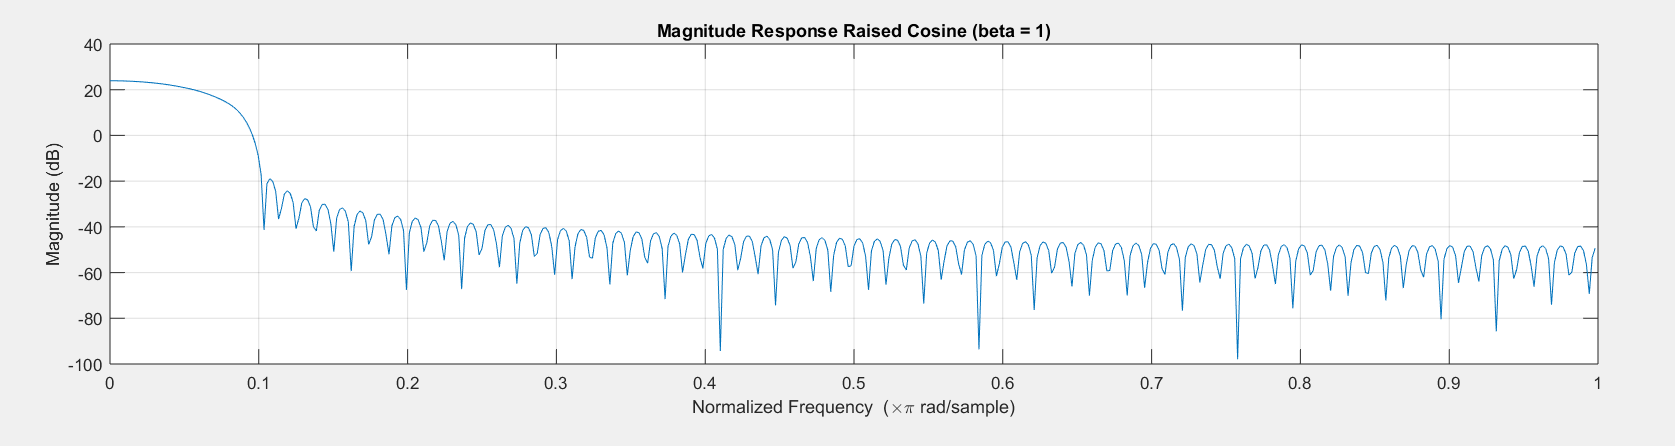
\includegraphics[width=\linewidth]{img/magnitude_response_beta_1.png}
      \caption{Magnitude Response $\beta = 1$}
    \end{subfigure}

    \begin{subfigure}[b]{0.5\linewidth}
      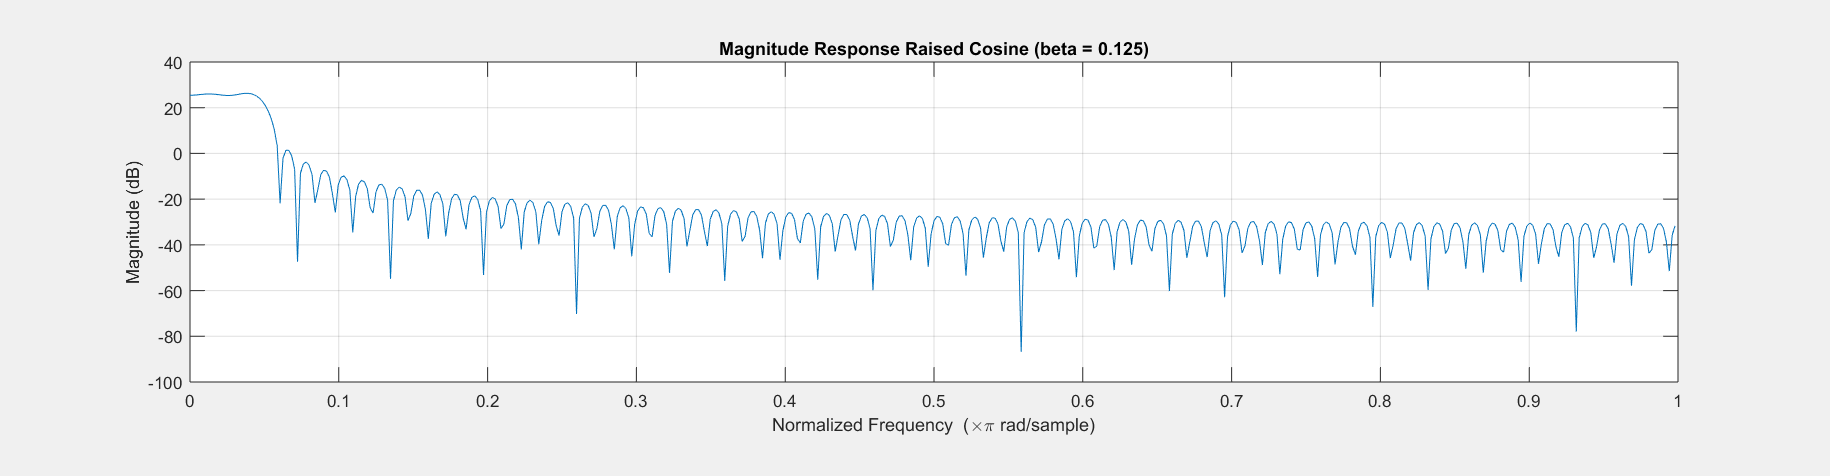
\includegraphics[width=\linewidth]{img/magnitude_response_beta_125.png}
      \caption{Magnitude Response $\beta = 0.125$}
    \end{subfigure}

  \end{center}
\end{figure}

\begin{figure}[h]
  \begin{center}

    \begin{subfigure}[b]{0.5\linewidth}
      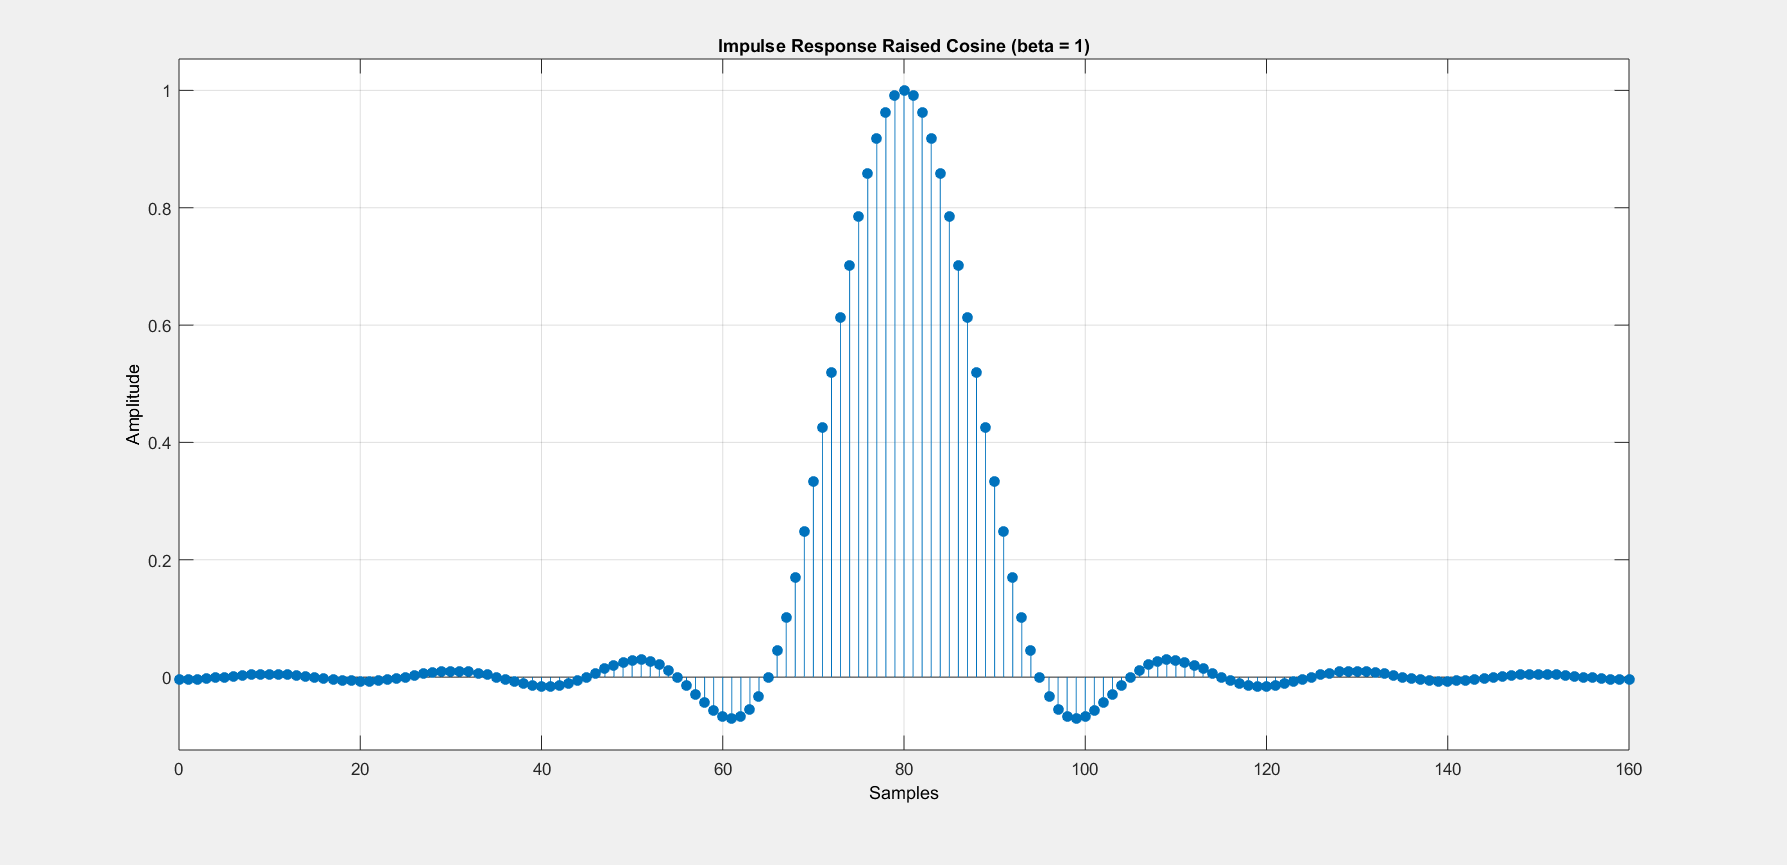
\includegraphics[width=\linewidth]{img/impulse_response_beta_1.png}
      \caption{Time Response $\beta = 1$}
    \end{subfigure}

    \begin{subfigure}[b]{0.5\linewidth}
      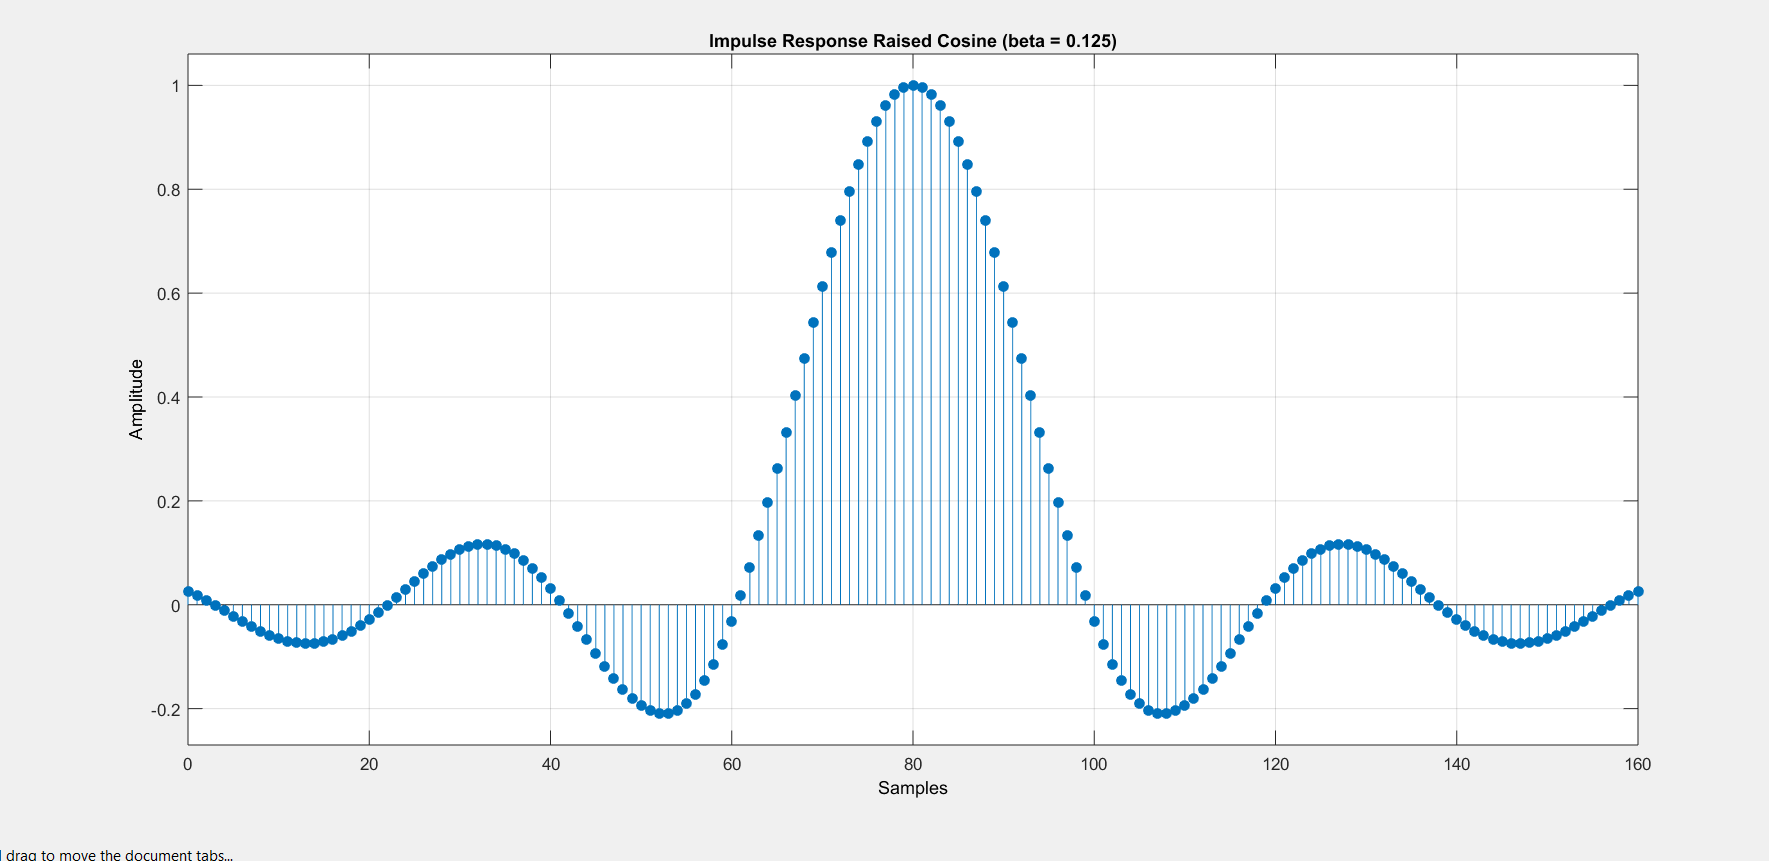
\includegraphics[width=\linewidth]{img/impulse_response_beta_125.png}
      \caption{Time Response $\beta = 0.125$}
    \end{subfigure}

  \end{center}
\end{figure}

Explain the major differences between the two filters with respect to their
	A) Magnitude responses 
	B) Impulse responses
2. What is the width of the impulse response for the =0.125 case? 
3. How would you obtain this number theoretically? (Hint: Look at the fsym and truncation limit you set)

\begin{figure}[h]
  \begin{center}

    \begin{subfigure}[b]{0.5\linewidth}
			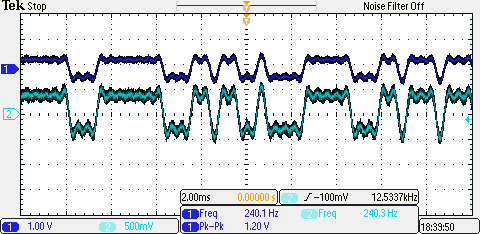
\includegraphics[width=0.65\textwidth]{img/DSK_implementation_beta_1.png}
      \caption{Time Response $\beta = 1$}
    \end{subfigure}

    \begin{subfigure}[b]{0.5\linewidth}
			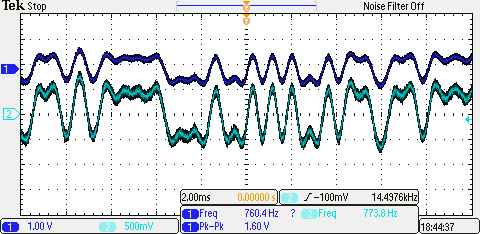
\includegraphics[width=0.65\textwidth]{img/DSK_implementation_beta_125.png}
      \caption{Time Response $\beta = 0.125$}
    \end{subfigure}

  \end{center}
\end{figure}

\subsection{Symbol Clock Recovery}

\textbf{Prefilter:}

\begin{center}
\begin{tabular}{c|c}
b0	&	 1				\\ \hline
b1	&  0				\\ \hline
b2	& -1				\\ \hline
-a1	&	 1.96004	\\ \hline
-a2	&	-0.984414 \\ \hline
\end{tabular}
\end{center}

\textbf{Bandpass:}

\begin{center}
\begin{tabular}{c|c}
b0	&	 1				\\ \hline
b1	&  0				\\ \hline
b2	& -1				\\ \hline
-a1	&	 1.87293\\ \hline
-a2	&	-0.969067\\ \hline
\end{tabular}
\end{center}

\begin{figure}[h]
  \begin{center}
    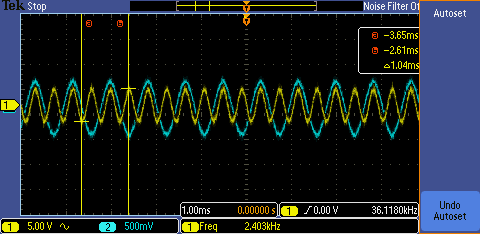
\includegraphics[width=0.65\textwidth]{img/dotting_sequence_SCR.png}
    \caption{Dotting sequence}
  \end{center}
\end{figure}

\begin{figure}[h]
  \begin{center}
    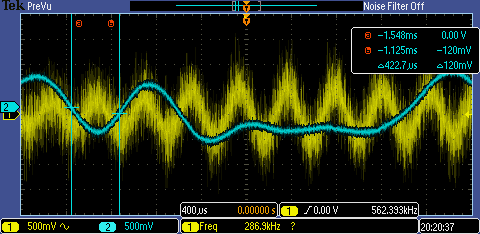
\includegraphics[width=0.65\textwidth]{img/2PAM_SCR.png}
    \caption{2-PAM SCR}
  \end{center}
\end{figure}

\pagebreak
\textbf{Code:}

\begin{verbatim}
	if (counter == 0) {
		symbol = SSRG_update(&SSRG_state); // pseudo random m-sequence
		x[0] = data[symbol]; // read the table

		/* dotting sequence
		symbol = symbol ^ 1;
		x[0] = data[symbol]; // read the table
		*/
	}

	// perform impulse modulation based on the FIR filter, B[N] 

	y  = 0;

	for (i = 0; i < 8; i++) {
		y +=  x[i]*B[counter + 20*i];	// perform the dot-product
	}

	if (counter == (samplesPerSymbol - 1)) {
		counter = -1; 

		/* shift x[] in preparation for the next symbol */

		for (i = 9; i > 0; i--) {
			x[i] = x[i - 1];          // setup x[] for the next input
		}
	}

	counter++;

	output = y;
	scr = clock_recover(y);
\end{verbatim}

\textbf{Table:}

\begin{center}
\begin{tabular}{c|c|c}
pattern	&	frequency & amplitude \\ \hline
dotted sequence	&	 2381 Hz	&	1.04 V				\\ \hline
dotted sequence	&	 2323 Hz	&	1.46 V				\\ \hline
\end{tabular}
\end{center}

\textbf{LPF:}

\begin{center}
\begin{tabular}{c|c}
b0	&	 1				\\ \hline
b1	&  1				\\ \hline
b2	&  0				\\ \hline
-a1	&	 0.509525\\ \hline
-a2	&	 0       \\ \hline
\end{tabular}
\end{center}

\textbf{Code:}

\begin{verbatim}
  if (counter == 0) {
		symbol = SSRG_update(&SSRG_state); // a faster version of rand() % 2
		x[0] = data[symbol]; // read the table
	}

  // perform impulse modulation based on the FIR filter, B[N] 
  y  = 0;

  for (i = 0; i < 8; i++) {
		y +=  x[i]*B[counter + 20*i];	// perform the dot-product
	}

  if (counter == (samplesPerSymbol - 1)) {
    counter = -1; 

		/* shift x[] in preparation for the next symbol */
 		for (i = 9; i > 0; i--) {
			x[i] = x[i - 1];          // setup x[] for the next input
		}
  }

  counter++;

	output = y*cosine[counter & 3];

	//receiver
	demod = 2*output*cosine[counter & 3];

	//LPF
	biquad_x[0][0] = demod;

	CodecDataOut.Channel[LEFT]  = y; // setup the LEFT  value
	CodecDataOut.Channel[RIGHT] = G[0] * biquad(0, biquad_x[0][0]); // setup the RIGHT value
\end{verbatim}

\begin{figure}[h]
  \begin{center}
    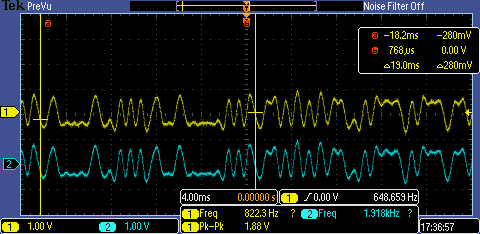
\includegraphics[width=0.65\textwidth]{img/tx_rx.png}
    \caption{transmit and recieve}
  \end{center}
\end{figure}

\begin{figure}[h]
  \begin{center}
    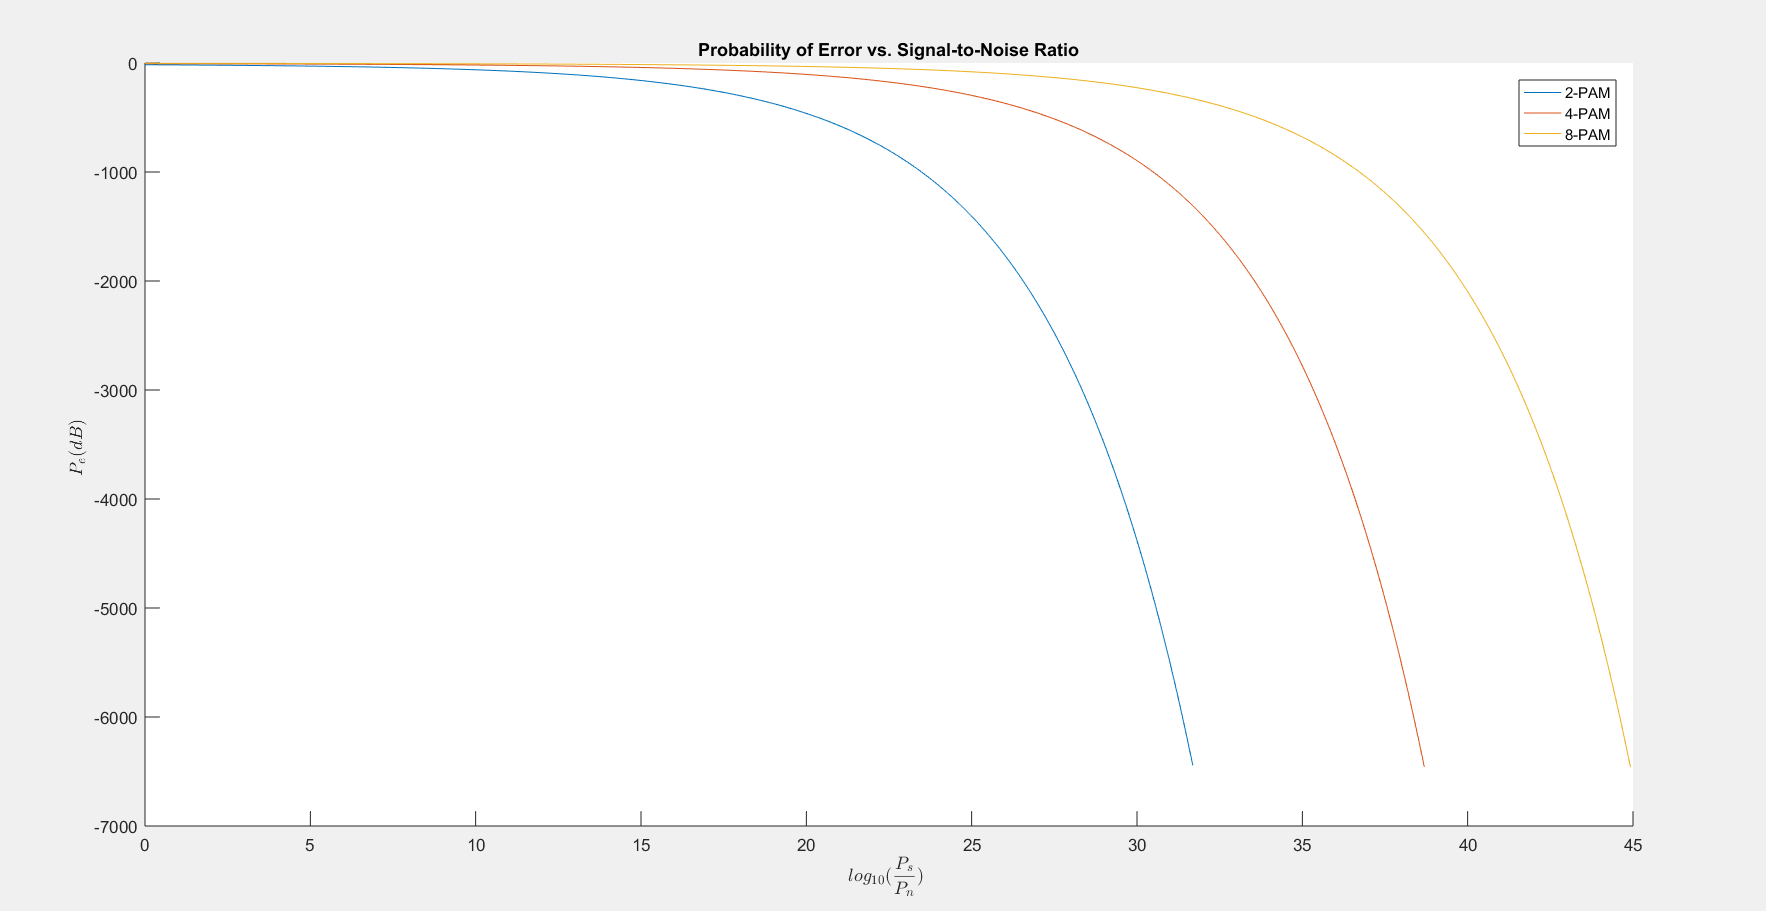
\includegraphics[width=0.65\textwidth]{img/probability_of_error.png}
    \caption{PES}
  \end{center}
\end{figure}

%----------------------------------------------------------------------------------------
%	SECTION 4
%----------------------------------------------------------------------------------------

\section{Discussion}


%----------------------------------------------------------------------------------------
%	SECTION 5
%----------------------------------------------------------------------------------------

\section{Answers to questions}

\begin{enumerate}
  \begin{item}
    Number of taps before you run out of time for FIR filtering.

  \textbf{Answer:}
    For an arbitrary processor using a circular buffer to implement an FIR filter, where $m$ is the time it takes for a multiply to complete and $a$ is the time it takes for an addition to complete.
    We would want our processing to take less than our sampling period $T_s$.
    So for an FIR filter with $N$ coefficients we  would have $N$ multiply and $N - 1$ add opperations.

    \begin{equation}
      T_s > mN + a(N - 1)
    \end{equation}

    Solving for $N$ we arrive at this constraint for the maximum number of taps.

    \begin{equation}
      \frac{T_s + a}{m + a} > N
    \end{equation}
  \end{item}

\end{enumerate}

%----------------------------------------------------------------------------------------
%	BIBLIOGRAPHY
%----------------------------------------------------------------------------------------

\bibliography{mybib}
\bibliographystyle{plain}

%----------------------------------------------------------------------------------------


\end{document}
